\section{Poetic parallelism}\label{sec:PoePar}
Another use of U\=/forms is in poetry.
In Amarasi poetry a semantically parallel pair of verbs
can also occur with complementary U\=/forms and M\=/forms.
An example is given in \qf{ex:130825-3, 1.21} below
in which the verb \ve{m-tenu} `shade (with umbrella)'
is both semantically and morphologically parallel
to the next verb \ve{mu-haof} `shade'.

\begin{exe}
	\ex{\glll	henatiʔ \bxA{m-te\tbr{nu}} =m \bxB{mu-ha\tbr{of}} too{\gap}tafaʔ =kai {\lks}\\
						henatiʔ {\gp}m-tenu =ma {\gp}mu-hafo too{\gap}tafaʔ =kai\\
						{\he} \gp\m-umbrella{\tbrU} =and \gp\muu-shade{\tbrM} citizen ={\kai}\\
			\glt	`So that you might shade [doublet] us people.'
						\txrf{130825-3, 1.21} {\emb{130825-3-01-21.mp3}{\spk{}}{\apl}}}\label{ex:130825-3, 1.21}
\end{exe}

Poetry in the Timor region makes extensive use of semantic parallelism.
Semantic parallelism is the pairing of related words or phrases to `say the same thing twice'.
Other terms used for this phenomenon include \emph{speaking in pairs}
and \emph{dyadic speech}, with the semantically paired words called a \emph{doublet}.
An English Biblical example from Isaiah 65:17--19 is given in
\qf{ex:Isaiah65:17-19} below, with doublets linked by connecting lines.

\begin{exe}
	\ex{\label{ex:Isaiah65:17-19}
		\begin{xlist}
			\exi{17}{
				\begin{xlist}
					\exi{a.}{\it{Behold, I will create new} \xytext{\fbox{\it{heavens}}\xybarconnect[2][-]{2}&\it{and a new}&\fbox{\it{earth.}}}}
					\exi{b.}{\it{The former things will not}\\ \xytext{\fbox{\it{be remembered,}}\xybarconnect[2][-]{2}&\it{nor will they}&\fbox{\it{come to mind.}}}}
				\end{xlist}}
			\exi{18}{
				\begin{xlist}
					\exi{a.}{\it{But} \xytext{\fbox{\it{be glad}}\xybarconnect[2][-]{2}&\it{and}&\fbox{\it{rejoice\vp{b}}}&}\it{forever in what I will create,}}
					\exi{b.}{\it{for I will create} \xytext{\fbox{\it{Jerusalem}}\hspace{-0.3em}\xybarconnect[2][-]{4}&\it{to be}\hspace{-0.3em}&\fbox{\it{a delight}}\hspace{-0.3em}\xybarconnect[4][-]{3}&\it{and}\hspace{-0.3em}&\fbox{\it{its people}}\hspace{-0.3em}&\fbox{\it{a joy.\vp{d}}}}}
				\end{xlist}}
		\end{xlist}}
\end{exe}
\newpage
\begin{exe}
	\sn{
		\begin{xlist}
			\exi{19}{
				\begin{xlist}
					\exi{a.}{\it{I will} \xytext{\fbox{\it{rejoice\vp{d}}}\hspace{-0.2em}\xybarconnect[2][-]{4}&\it{over}\hspace{-0.2em}&\fbox{\it{Jerusalem}}\hspace{-0.2em}\xybarconnect[4][-]{4}&\it{and}&\fbox{\it{take delight}}\hspace{-0.2em}&\it{in}\hspace{-0.2em}&\fbox{\it{my people;}}}}
					\exi{b.}{\it{the sound of} \xytext{\fbox{\it{weeping}}\hspace{-0.2em}\xybarconnect[2][-]{2}&\it{and of}&\fbox{\it{crying}}\hspace{-0.2em}&}\it{will be heard in it no more.}}
				\end{xlist}}
		\end{xlist}}
\end{exe}

Each verse is divided into two parts, each of which contains at least one doublet.
In some cases the words are opposites,
such as the pair \it{heavens‖earth} in verse 17,
but more often the pairs are of words or phrases which mean similar things,
such as the pair \it{weeping‖crying} in verse 19.
The members of such pairs are effectively synonymous
when used as a doublet even if they are not exact synonyms
when used individually in other contexts.

A specific kind of semantic parallelism is canonical parallelism.
Canonical parallelism is a circumscribed system of semantic parallelism
in which the words and phrases which may form pairs are pre-defined.
In such a system speakers are not free to innovate new pairs.

Canonical parallelism has been extensively studied in eastern Indonesia by James Fox
(see particularly \citealt{fo88,fo14})
who has been especially interested in poetry of the island of Rote,
neighbouring the Timor mainland where Meto is spoken.
An example of Rote parallelism is given in \qf{ex:RotPar} below.
This example consists of the first six lines of a particular chant.
Each pair of lines contains three words
each of which is paired with another word in the next line.

\begin{exe}\let\eachwordone=\itshape
	\ex{Poetic parallelism in Rote:\footnote{
		Each pair of lines has been combined into a single typed line in \qf{ex:RotPar}
		to show clearly the links between paired words.
		Morpheme breaks are not shown to reduce clutter.}
	\hfill{\cite[76f]{fo74}}\vspace{16pt}}\label{ex:RotPar}
	\begin{xlist}
		\ex{\gll \bxA{lole\vp{f}} \bxB{faik\vp{f}} \bxX{ia\vp{f}} \rnode{C}{\psframebox[linewidth=0.4pt]{dalen\vp{f}}} \bxX{ma\vp{f}} \rnode{D}{\psframebox[linewidth=0.4pt]{lada\vp{f}}} \rnode{E}{\psframebox[linewidth=0.4pt]{ledok\vp{f}}} \bxX{ia\vp{f}} \rnode{F}{\psframebox[linewidth=0.4pt]{tein\vp{f}}} \bxX{naa\vp{f}} 
							{\ncbar[arm=5pt,angle=90,linewidth=0.4pt]{-}{A}{D}}{\ncbar[arm=10pt,angle=90,linewidth=0.4pt]{-}{B}{E}}{\ncbar[arm=15pt,angle=90,linewidth=0.4pt]{-}{C}{F}}
							\\
						 {\gp}good {\gp}day {\gp}this {\gp}inside {\gp}and {\gp}fine {\gp}time {\gp}this {\gp}stomach {\gp}that \\
		\glt	`On this good day, and at this fine time.'\vspace{16pt}}
		\ex{\gll \bxX{lae:\vp{f}} \bxA{tefu} \bxB{maŋgona\vp{f}} \rnode{C}{\psframebox[linewidth=0.4pt]{lilok\vp{f}}} \bxX{ma\vp{f}} \rnode{D}{\psframebox[linewidth=0.4pt]{huni\vp{f}}} \rnode{E}{\psframebox[linewidth=0.4pt]{malapa\vp{f}}} \rnode{F}{\psframebox[linewidth=0.4pt]{losik\vp{f}}}{\ncbar[arm=5pt,angle=90,linewidth=0.4pt]{-}{A}{D}}{\ncbar[arm=10pt,angle=90,linewidth=0.4pt]{-}{B}{E}}{\ncbar[arm=15pt,angle=90,linewidth=0.4pt]{-}{C}{F}}
							\\
						 {\gp}say sugarcane {\gp}sheathed {\gp}gold {\gp}and {\gp}banana {\gp}blossomed {\gp}copper\\
		\glt	`They say: the sugarcane has sheaths of gold, and the banana has blossoms of copper.'\vspace{11pt}}
		\ex{\gll \bxA{tefu} \bxB{olu\vp{f}} \bxX{heni\vp{f}} \rnode{C}{\psframebox[linewidth=0.4pt]{ŋgonan\vp{f}}} \bxX{ma\vp{f}} \rnode{D}{\psframebox[linewidth=0.4pt]{huni\vp{f}}} \rnode{E}{\psframebox[linewidth=0.4pt]{kono\vp{f}}} \bxX{heni\vp{f}} \rnode{F}{\psframebox[linewidth=0.4pt]{lapan\vp{f}}}
							{\ncbar[arm=5pt,angle=90,linewidth=0.4pt]{-}{A}{D}}{\ncbar[arm=10pt,angle=90,linewidth=0.4pt]{-}{B}{E}}{\ncbar[arm=15pt,angle=90,linewidth=0.4pt]{-}{C}{F}}\\
						sugarcane shed {\gp}away {\gp}sheath {\gp}and banana {\gp}fall {\gp}away blossom\\
		\glt	`The sugarcane sheds its sheath, and the banana drops its blossom.'}
	\end{xlist}
\end{exe}

Poetry in Amarasi also employs semantic parallelism.
Traditionally, Amarasi also uses canonical parallelism.
%though some modern poets innovate beyond the constraints of this pre-defined system.
Not only are the words which can form doublets fixed,
but the order in which each member of a doublet occurs is also fixed.
Other features of Amarasi poetry include the use of metaphor, archaisms,
and a preference for morphologically complex words.

An example of Amarasi parallelism is given in \qf{ex:140726 0.00--0.14}
below, which consists of the first part of a traditional chant.
Such greetings are known as \ve{aʔa srama-t} (poetic.speech greet-{\at}) in Amarasi.
Every second line (those in capital letters) repeats one
of the phrases from the previous line and is said by the whole group.
The other lines are spoken by the group leader.

\begin{exe}
	\ex{Amarasi chant (\ve{aʔa sramat}): \txrf{140726}{\emb{140726-00-00-00-14.mp3}{\spk{}}{\apl}}\vspace{5pt}}\label{ex:140726 0.00--0.14}
	\begin{xlist}
		\ex{\gll	\bxA{baisenu-t} =ma \bxB{ronaen} n-eu \rnode{C}{\psframebox[linewidth=0.4pt]{mutiʔ}} =ma \rnode{D}{\psframebox[linewidth=0.4pt]{mnatuʔ}} et
							{\lks} {\ncbar[arm=5pt,angle=90,linewidth=0.4pt]{-}{C}{D}}\\
							{\gp}look.up =and {\gp}greeting \n-{\eu} {\gp}silver =and {\gp}gold {\et} \\ \vspace{5pt}}
		\sn{\gll	\bxA{muit} ma-hine-ʔ =ma \bxB{mnatuʔ} neee {\lks}\\
							{\gp}silver {\ma}-know-{\ma} =and {\gp}gold \tsc{pause}\\
				\glt	`Greetings and honour to all people, who are like silver and gold, wise, and knowledgeable silver and gold,' \txrf{0.00}}
		\ex{\gll	MA-HINE-Ɂ \\
							{\ma}-know-{\ma} \\
				\glt	`So wise.'	\txrf{0.05}}
		\ex{\gll	n-eu \bxA{a-ʔnae-t} =ma \bxB{a-mepu-t} a|n-bi Uisneno iin meupg=aa =m neee {\lks}\\
							\n-{\eu} \gp\at-great-{\at} =and \gp\at-work-{\at} \a\n-{\bi} God {\iin} work={\aa} =and \tsc{pause}\\
				\glt	`to the leaders and workers serving in God's work,' \txrf{0.07}}
		\ex{\gll	RO MEPU \\
							truly work \\
				\glt `Truly working.'\txrf{0.10}\vspace{5pt}}
		\ex{\gll	na-tuin \bxA{sarit} =ma \bxB{bekot} a-reok-t =aa =m neee {\lks}\\
							\na-follow {\gp}intention =and {\gp}plan {\at}-good-{\at} ={\aa} =and \tsc{pause}\\
				\glt	`following (His) good intentions and plans,' \txrf{0.12}}
		\ex{\gll	A-REKO-T \\
							{\at}-good-{\at}\\
				\glt `So good.'\txrf{0.14}}
	\end{xlist}
\end{exe}

When an Amarasi doublet consists of two verbs and
the connector \ve{=ma} `and' occurs between them,
it is usual for the first verb to take the M\=/form.
This is consistent with the use of M\=/forms before \ve{=ma}
as discussed in \srf{sec:Mfo=Ma},
in which each verb encodes a single event rather than two discrete events.
Three examples of verbal doublets with an initial M\=/form
are given in \qf{ex:130825-3, 0.51}--\qf{ex:Romans 9:13} below.

\begin{exe}
		\ex{\glll	hai mi-ʔ-futu-ʔ =kii ʔ-fuut nafe, henatiʔ \\
							hai mi-ʔ-futu-ʔ =kii ʔ-futu-ʔ nafe henatiʔ  \\
							{\hai} \mi-\qV-tie-{\qV} ={\kii} \qq-tie belt {\he} \\ \vspace{5pt}}
		\sn{\glll	\bxA{m-fu\tbr{ut}} =ma \bxB{m-nibun} m-aan too{\gap}tafaʔ =kai {\lks}\\
							{\gp}m-futu =ma {\gp}m-nibun m-ana too{\gap}tafaʔ =kai\\
							\gp\m-tie{\tbrM} =and \gp\m-surround \m-{\ana} citizen ={\kai}\\
				\glt	`We clothe you with a cloth belt so that you will surround and bind us people together.'
							\txrf{130825-3, 0.51} {\emb{130825-3-00-51.mp3}{\spk{}}{\apl}}}\label{ex:130825-3, 0.51}
		\ex{\glll	hai aaʔ-t=ii \bxA{na-m-so\tbr{up}} =ma \bxB{n-heun-ʔ=oo-n} on naan nai tua. {\lks}\\
							hai aʔa-t=ii {\gp}na-m-sopu =ma {\gp}n-henu-ʔ=oo-n on naan nai tua.\\
							{\hai} poetry-{\at}={\ii} \gp\na-\mv-finish{\tbrM} =and \gp\n-fill{\Mv}-{\qV}={\oo}-{\N} like {\naan} already {\tua}\\
				\glt	`Our poetry is now finished and complete like that.'
							\txrf{130825-3, 2.35} {\emb{130825-3-02-35.mp3}{\spk{}}{\apl}}\vspace{5pt}}
	\ex{\glll	mes au ka= \bxA{ʔ-si\tbr{um}} =ma \bxB{ʔ-toup} =fa naiʔ Esau. {\lks}\\
						mes au ka= {\gp}ʔ-simo =ma {\gp}ʔ-topu =fa naiʔ Esau\\
						but {\au} {\ka}= \gp\q-receive{\tbrM} =and \gp\q-receive{\M} ={\fa} {\naiq} Esau\\
			\glt	`But I did not receive [doublet] Esau.' \txrf{Romans 9:13}}\label{ex:Romans 9:13}
\end{exe}

However, it is also possible for the first verb of the doublet
to occur in the U\=/form with the second verb in the M\=/form.
One example is given in \qf{ex:120715-0, 0.45-0.58} below.

\newpage
\begin{exe}
	\ex{Greeting (\ve{aʔa sramat}): \txrf{120715-0} {\emb{120715-0-00-51-00-58.mp3}{\spk{}}{\apl}}}\label{ex:120715-0, 0.45-0.58}
	\begin{xlist}
		\ex{\glll	iin tua-n=ee ees--, ees naiʔ Bani, naiʔ Oraʔ, \\
							ini tua-n=ee {} esa naiʔ Bani naiʔ Oraʔ \\
							{\iin} owner-\N={\ee} {} one {\naiq} Bani {\naiq} Ora{\Q} \\}
		\vspace{4pt}
		\sn{\glll	\bxA{n-si\tbr{mo}} =ma \bxB{n-to\tbr{up}} tuaf am-nema-t \sf{tamu} neee {\lks} \\
							{\gp}n-simo =ma {\gp}n-topu tuaf am-nema-t \sf{tamu} neee \\
							\gp\n-receive{\tbrU} =and \gp\n-receive{\tbrM} person {\at}-come-{\at} guest \tsc{pause} \\
				\glt	`Its lords the Bani and Ora{\Q} clans receive [doublet] those who come (and those who are) guests.'
							\txrf{0.51}}\label{ex:120715-0, 0.51}
		\ex{\ve{AMNEMAT} \txrf{0.58}}
	\end{xlist}
\end{exe}

In \qf{ex:120715-0, 0.45-0.58} the U\=/form \ve{ʔ-simo} is paired with M\=/form \ve{ʔ-toup} `receive'.\footnote{
		The normal word for `receive' in Amarasi is \ve{topu},
		with \ve{simo} only occurring in poetic parallelism.
		The verb \ve{simo} is from another variety of Meto
		in which this is the normal word for `receive'
		-- a common strategy to create parallel pairs \citep[27f]{grth97}.}
		%Another example can be seen in the pair
		%\ve{amnemat‖tamu} `those who come ‖ guests'
		%also in \qf{ex:120715-0, 0.51} in which the second member
		%is a borrowing from Malay \it{tamu} `guest'.}
Another example of the same pair with
alternate U\=/form and M\=/forms is given in \qf{ex:OurLovGen} below,
a prayer composed and written by my main consultant Roni.
A scan of the original is given in Figure \ref{fig:OffPra} following.

\begin{exe}
	\ex{Prayer for the offertory collected in Church: \txrf{}}\label{ex:OurLovGen}
	\begin{xlist}
		\ex{\gll	a-ma-hoe-t a-ma-neka-t hai usiʔ, \\
							{\at}-{\ma}-bless-{\at} {\at}-{\ma}-love-{\at} {\hai} lord,\\
				\glt	`Our loving and generous lord,'}
		\ex{\gll	a|n-bi Yesus Kristus fuaʔturu ʔhonis. \\
							{\a\n}-{\bi} Jesus Christ offering living\\
				\glt	\lh{a|}`in (the name of) Jesus Christ, the living sacrifice.'}
		\ex{\glll	hai m-nonaʔ =ma m-fee fuaʔturuʔ reʔ hai \\
							hai m-nonaʔ =ma m-fee fuaʔturuʔ reʔ hai \\
							{\hai} {\m}-hand{\Uc} =and {\m}-give offering {\req} {\hai} \\ \vspace{5pt}}
		\sn{\glll	\bxA{n-si\tbr{mo}} =ma \bxB{n-to\tbr{up}} =siin mi-ʔko {\lks}\\
							{\gp}n-simo =ma {\gp}n-topu =siin mi-ʔko \\
							\gp\n-receive{\tbrU} =and \gp\n-receive{\tbrM} ={\siin} {\mi}-{\qko} \\}
		\sn{\glll	hoo ʔnima-m a-ma-neka-b, {\lks}\\
							hoo ʔnima-m a-ma-neka-b,\\
							{\hoo} hand-{\mg} {\at}-{\ma}-love-{\b}\\
				\glt	`We give offerings we received from your loving hand.'}
		\ex{\gll	ka= baʔ{\tl}bauʔk=ein =fa, fuʔ{\tl}fuʔan na-heun n-ok rahi oe{\gap}metan,\\
							{\ka}=  {\prd}many={\ein} ={\fa} {\prd}few \na-full{\M} \n-{\ok\M} filth dirt\\
				\glt	`(It's) not very much, (but) very little (and) filled with filth and dirt,' }
		\ex{\gll	mes hai m-eik =siin m-eu =koo usi, m-eik Yesus iin kana-n.\\
							but {\hai} \m-bring{\M} ={\siin} \m-{\eu} ={\koo} Lord \m-bring{\M} Jesus {\iin} name-{\N}\\
				\glt	`but we bring them to you Lord, in Jesus's name.' }
	\end{xlist}
\end{exe}

\begin{figure}[h]
	\caption{Prayer for the offertory collected in church}\label{fig:OffPra}%
	\centering\setlength\fboxsep{-0.5pt}\setlength\fboxrule{0.75pt}
		\fbox{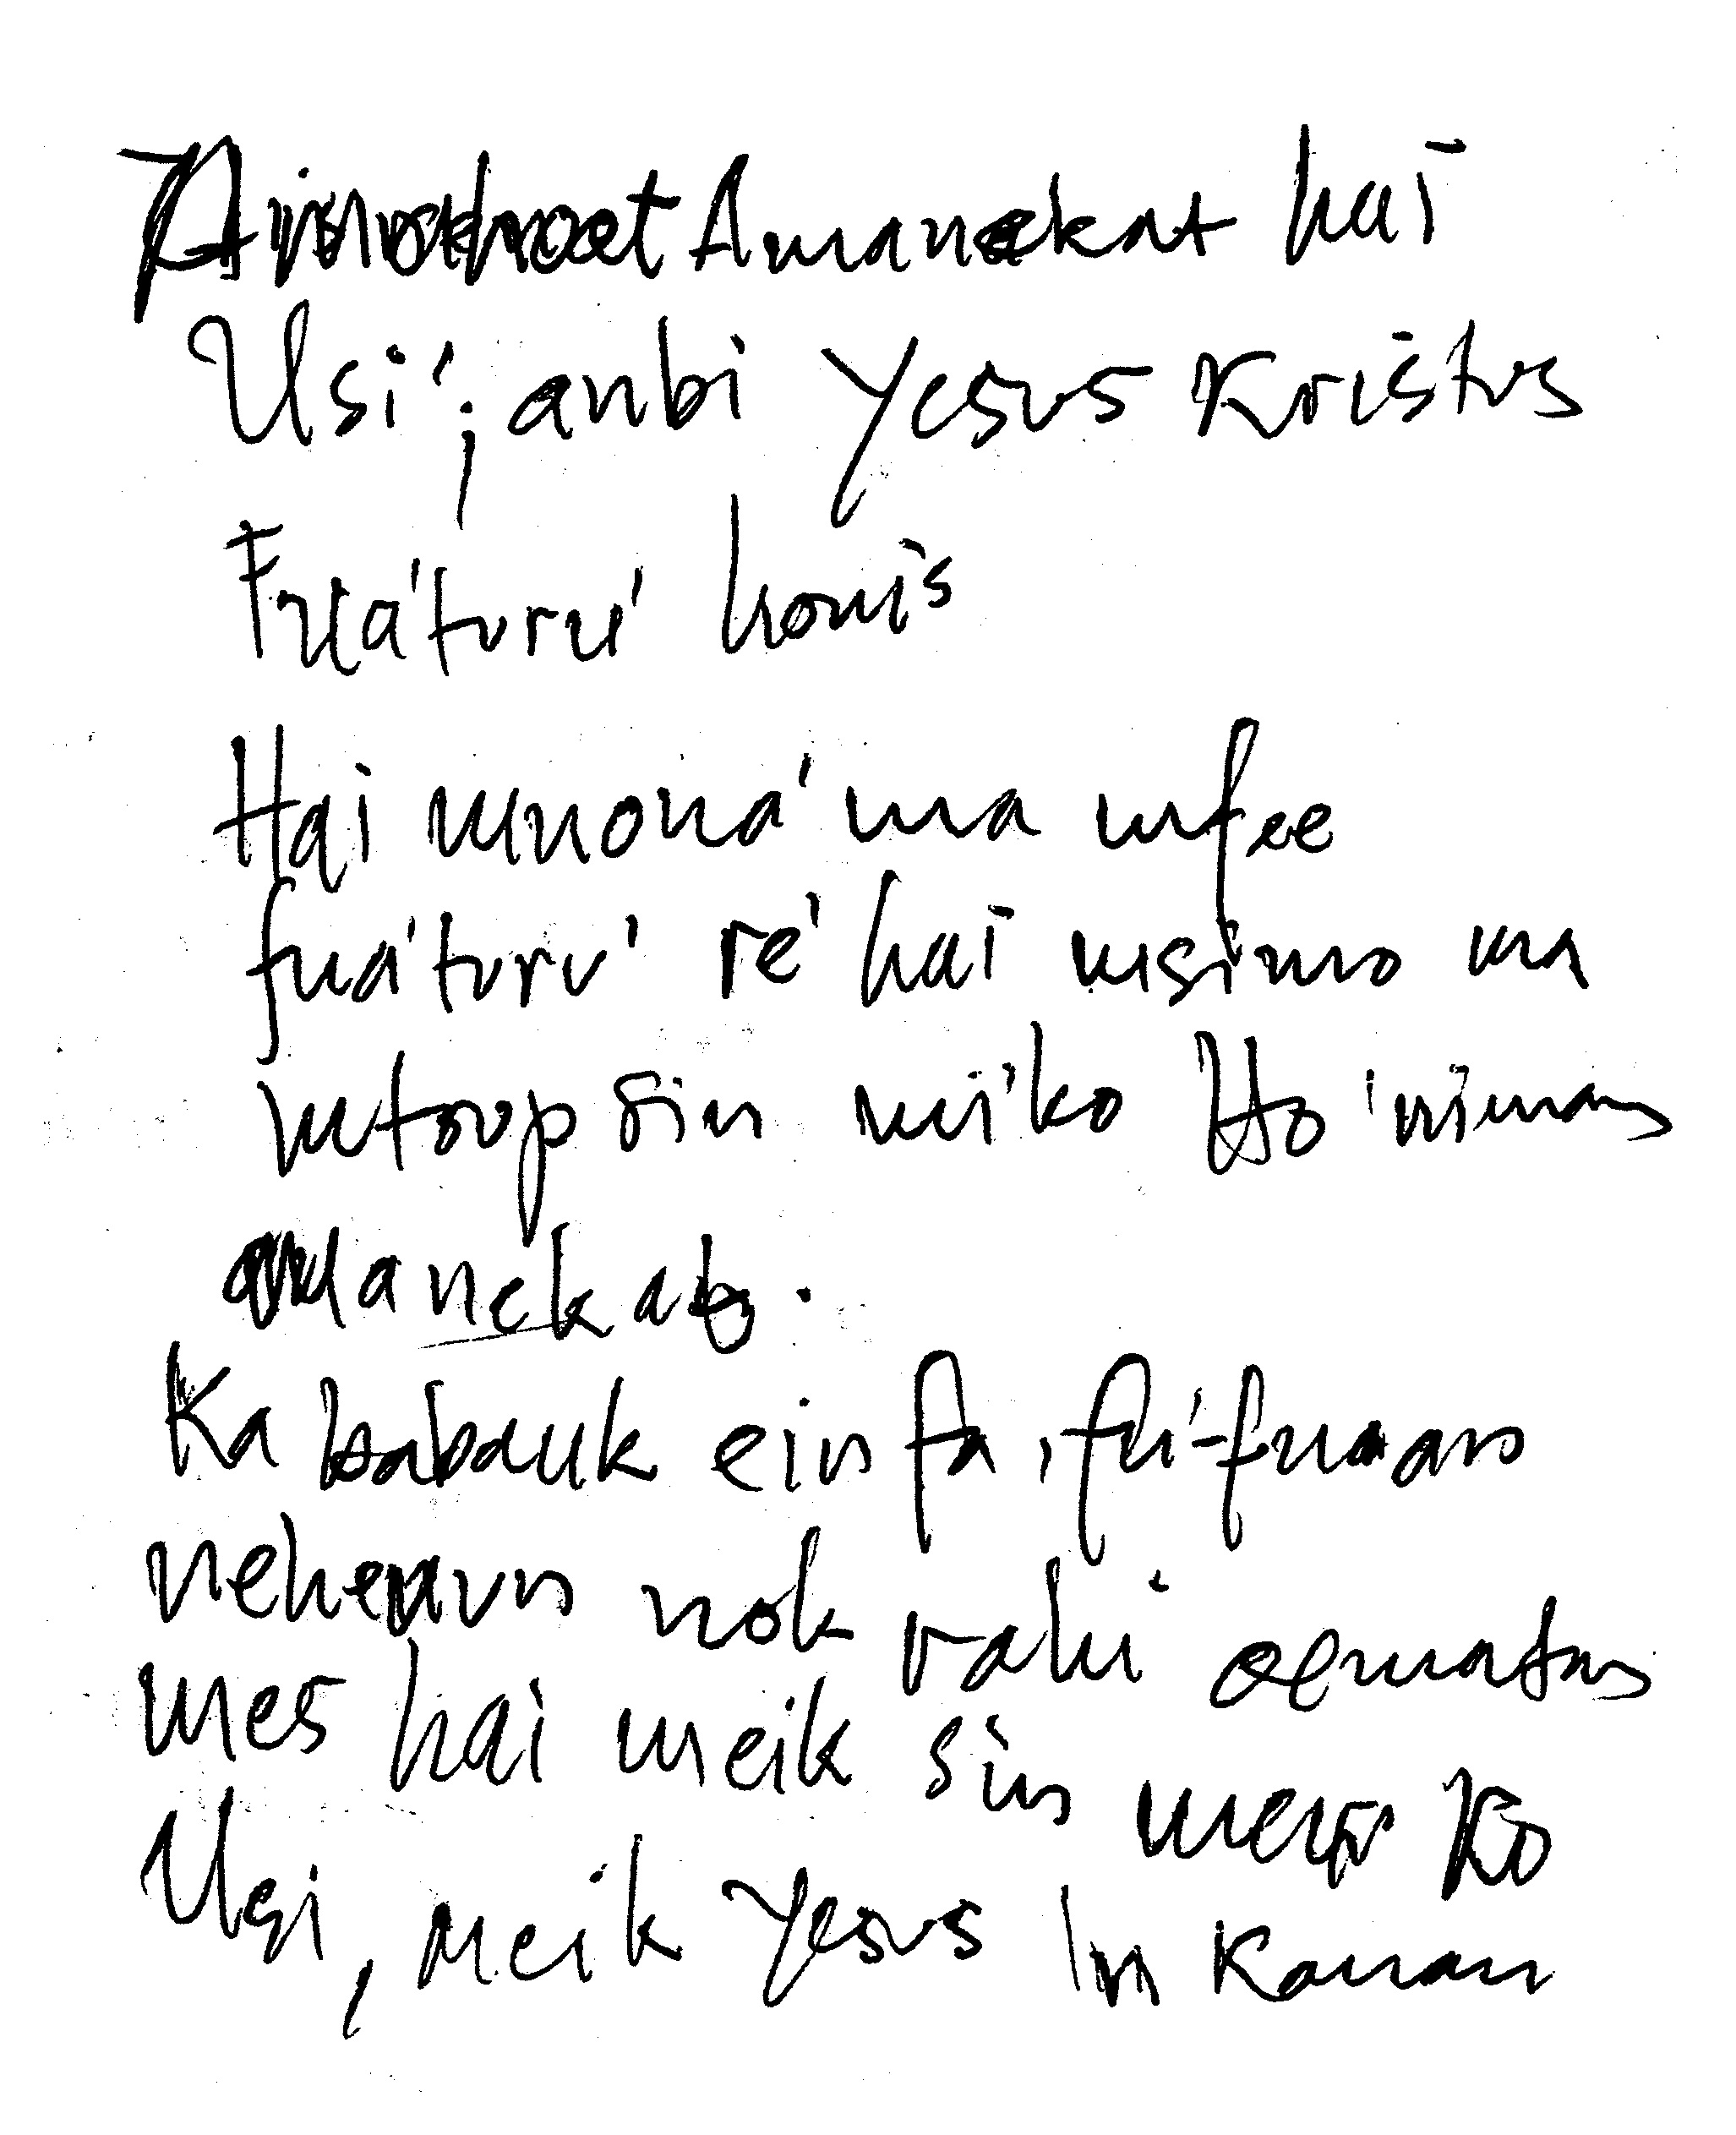
\includegraphics[width=0.6\columnwidth]{aaz-nodate-OffertoryPrayer.jpg}}
\end{figure}

A third example of parallel verbs with an alternate U\=/form and M\=/form
is given in \qf{ex:130825-3, 1.15-1.21}.
In this case the doublet is \ve{tenu \tcb{‖} hafo} `umbrella : shade'.

\newpage
\begin{exe}
	\ex{Speech to welcome new government officials:
				\txrf{130825-3} {\emb{130825-3-01-15-01-21.mp3}{\spk{}}{\apl}}}\label{ex:130825-3, 1.15-1.21}
	\begin{xlist}
		\ex{\glll	hai mi-ʔpiruʔ =kii ʔpiur suun mees nua\\
							hai mi-ʔpiruʔ =kii ʔpiruʔ suna meseʔ nua\\
							{\hai} {\mi}-cloth{\Uc} ={\kii} cloth horn single two\\
				\glt	`We give you two single bandannas (as a) horn' \txrf{1.15}}\vspace{4pt}
		\ex{\glll	henatiʔ \bxA{m-te\tbr{nu}} =m \bxB{mu-ha\tbr{of}} too{\gap}tafaʔ =kai {\lks}\\
							henatiʔ {\gp}m-tenu =ma {\gp}mu-hafo too{\gap}tafaʔ =kai\\
							{\he} \gp\m-umbrella{\tbrU} =and \gp\muu-shade{\tbrM} citizen ={\kai}\\
				\glt	`so that you might shade [doublet] us people.' \txrf{1.21}}
	\end{xlist}
\end{exe}

The two main patterns in which an Amarasi poetic doublet
of parallel verbs occur are given
in \qf{ex:AmaParVerPai} and \qf{ex:AmaParVerPai2} below.

\begin{exe}
	\ex{\xytext{\fbox{verb\sub{1}{\M}}\xybarconnect[2][-]{2}&and&\fbox{verb\sub{2}{\M}}}}\label{ex:AmaParVerPai}
	\ex{\xytext{\fbox{verb\sub{1}{\U}}\xybarconnect[2][-]{2}&and&\fbox{verb\sub{2}{\M}}}}\label{ex:AmaParVerPai2}
\end{exe}

In non-poetic discourse the use of a U\=/form followed by \ve{=ma}
indicates that the event marked by the U\=/form preceded the
event encoded in the next clause, as discussed in \srf{sec:Coo=Ma}.
However, in poetry such U\=/forms do not indicate the timing of events.
Instead, the use of U\=/forms and M\=/forms is a poetic device,
providing the option of a double parallelism on complementary verbs;
such verbs are both semantically and morphologically parallel.
